\documentclass[10pt,utf8,presentation,notheorems,xcolor=dvipsnames,compress]{beamer}
\usepackage{doclad}

%Тут можно вставить дополнительные пакеты

\title[Создание интерфейса к БД]{
Создание интерфейса пользователя \newline к БД «кафедральная нагрузка»
}

\author[Ромакина О.М.]{
  Ромакина Оксана Михайловна
}



\date{06 июня  2014}

\begin{document}

\begin{frame}
\titlepage
\end{frame}

\section<presentation>*{Содержание}

\begin{frame}
\frametitle{Содержание}
\tableofcontents
\end{frame}

\section{Введение}
\begin{frame}
\frametitle{Введение}
\begin{block}{Планирование работы кафедры.}
Максимальную трудоемкость с точки зрения планирования учебного процесса на кафедре представляет распределение
учебной нагрузки текущего года
\end{block}
\begin{block}{БД «кафедральная нагрузка»}
разработана сотрудниками кафедры. В качестве СУБД использовалась БД \emph{PostgreSQL}. 
В качестве  интерфейса пользователя применялась \emph{Knoda}.
\end{block}
\begin{block}{Основная идея дипломной работы}
Применить для разработки интерфейса пользователя 
модуль \emph{PyQt4} языка \emph{Python} для построения
интерфейса пользователя к БД «кафедральная нагрузка».
\end{block}
\end{frame}

\section{Структура БД «кафедральная нагрузка»}

\subsection{Описание СУБД PostgreSQL}
\begin{frame}
\frametitle{Описание СУБД PostgreSQL}

\begin{block}{PostgreSQL}
это объектно-реляционная база данных
\end{block}

\begin{block}{PostgreSQL}
это программный продукт с открытым исходным кодом и свободной лицензией.
\end{block}
\end{frame}

\section{Структура БД «кафедральная нагрузка»}
\begin{frame}
\frametitle{Группы/подгруппы/потоки}
Структура БД «кафедральная нагрузка» была разработана
сотрудниками кафедры. Ниже представлена структура БД.
\begin{center}
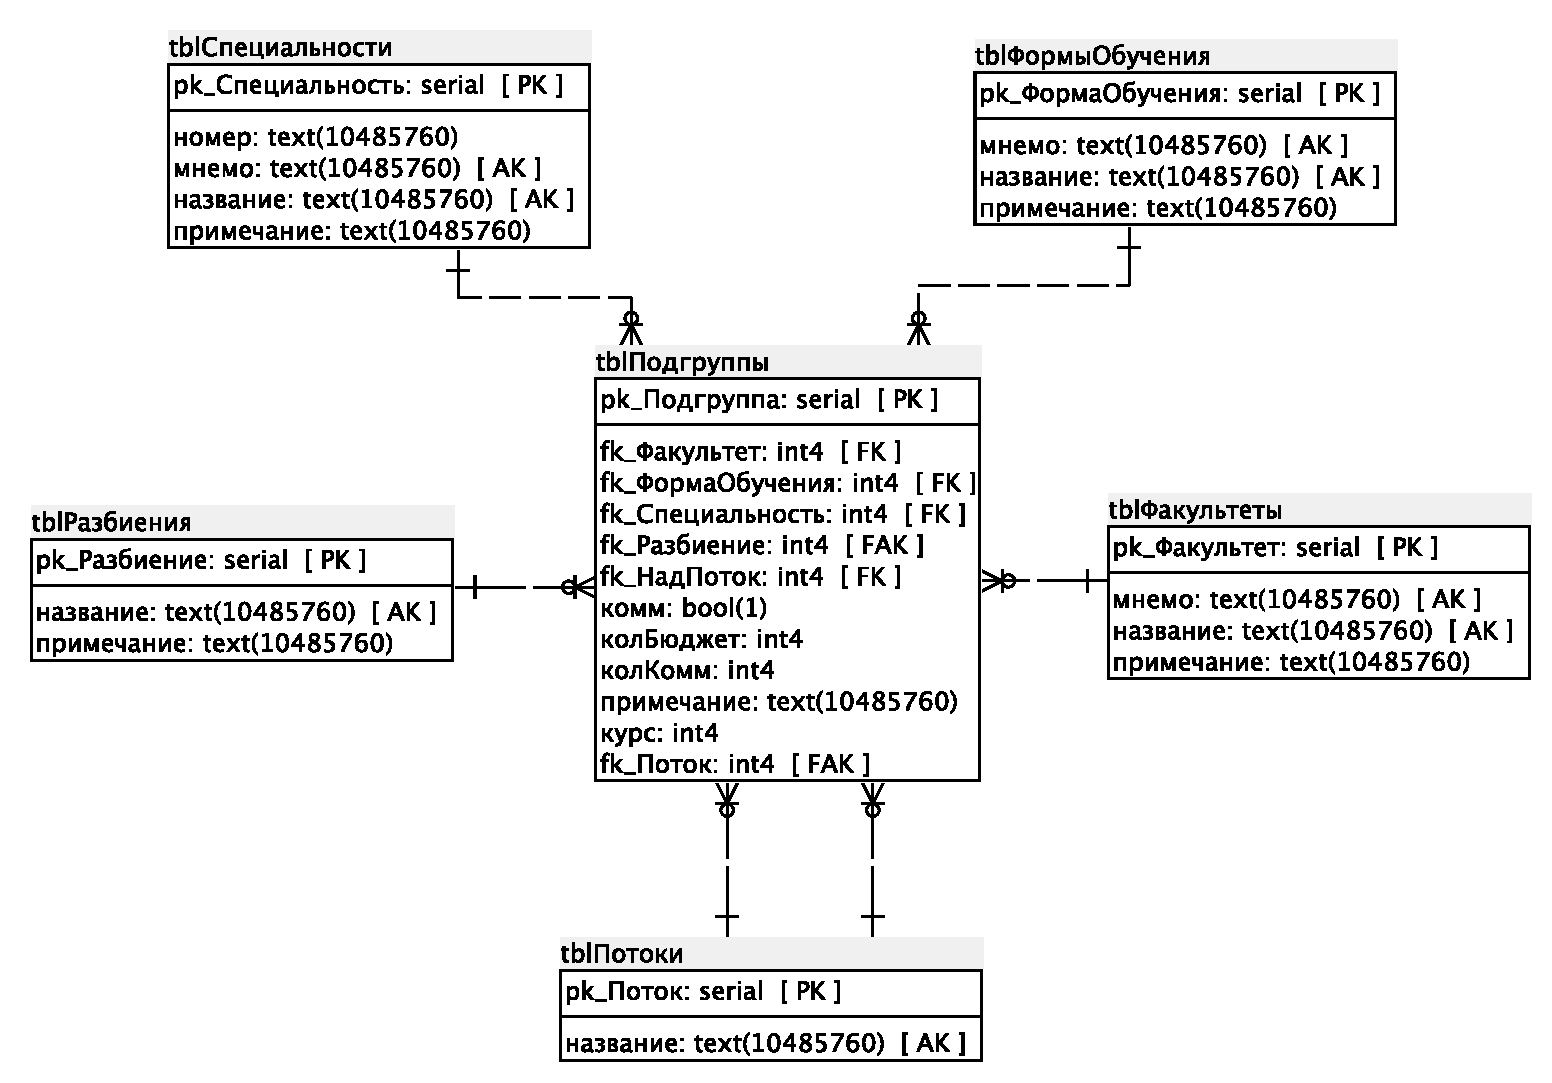
\includegraphics[scale=0.35]{db1}%
\end{center}
\end{frame}

\begin{frame}
\frametitle{Преподаватели/заявки}
\begin{center}
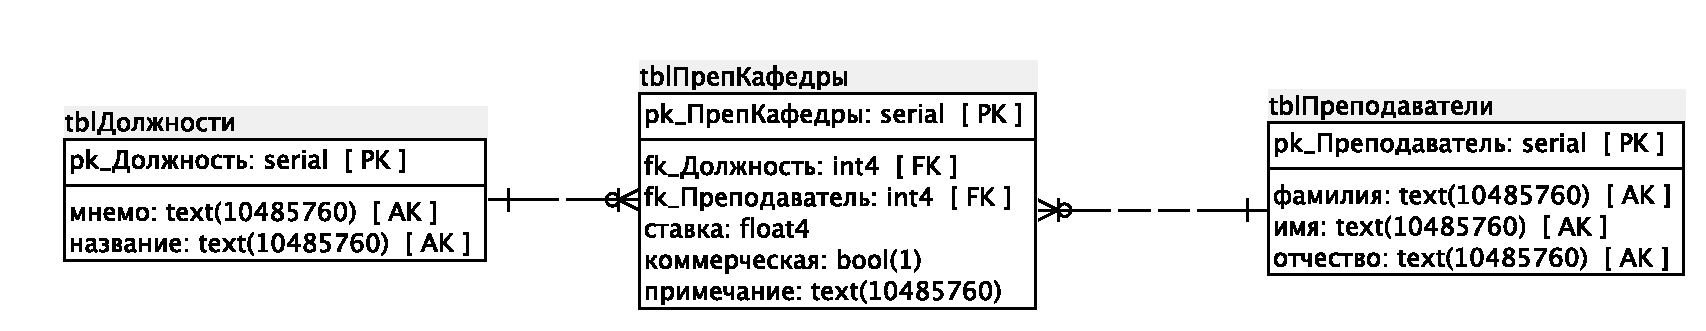
\includegraphics[scale=0.4]{db2}\\
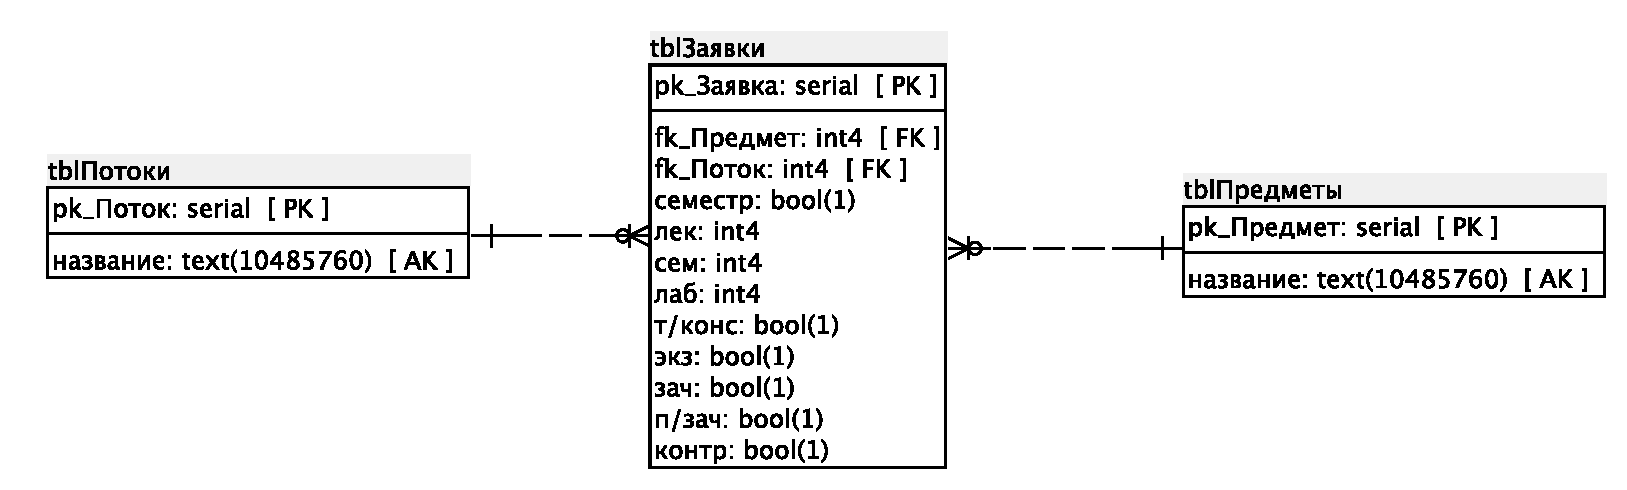
\includegraphics[scale=0.4]{db3}\\
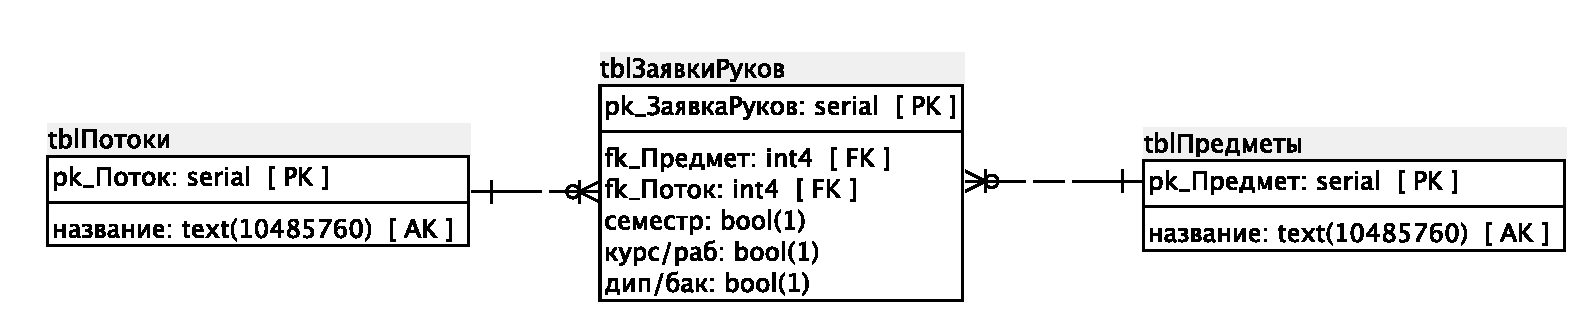
\includegraphics[scale=0.4]{db4}%
\end{center}
\end{frame}

\begin{frame}
\frametitle{Нагрузка}
\begin{center}
\vskip -1cm
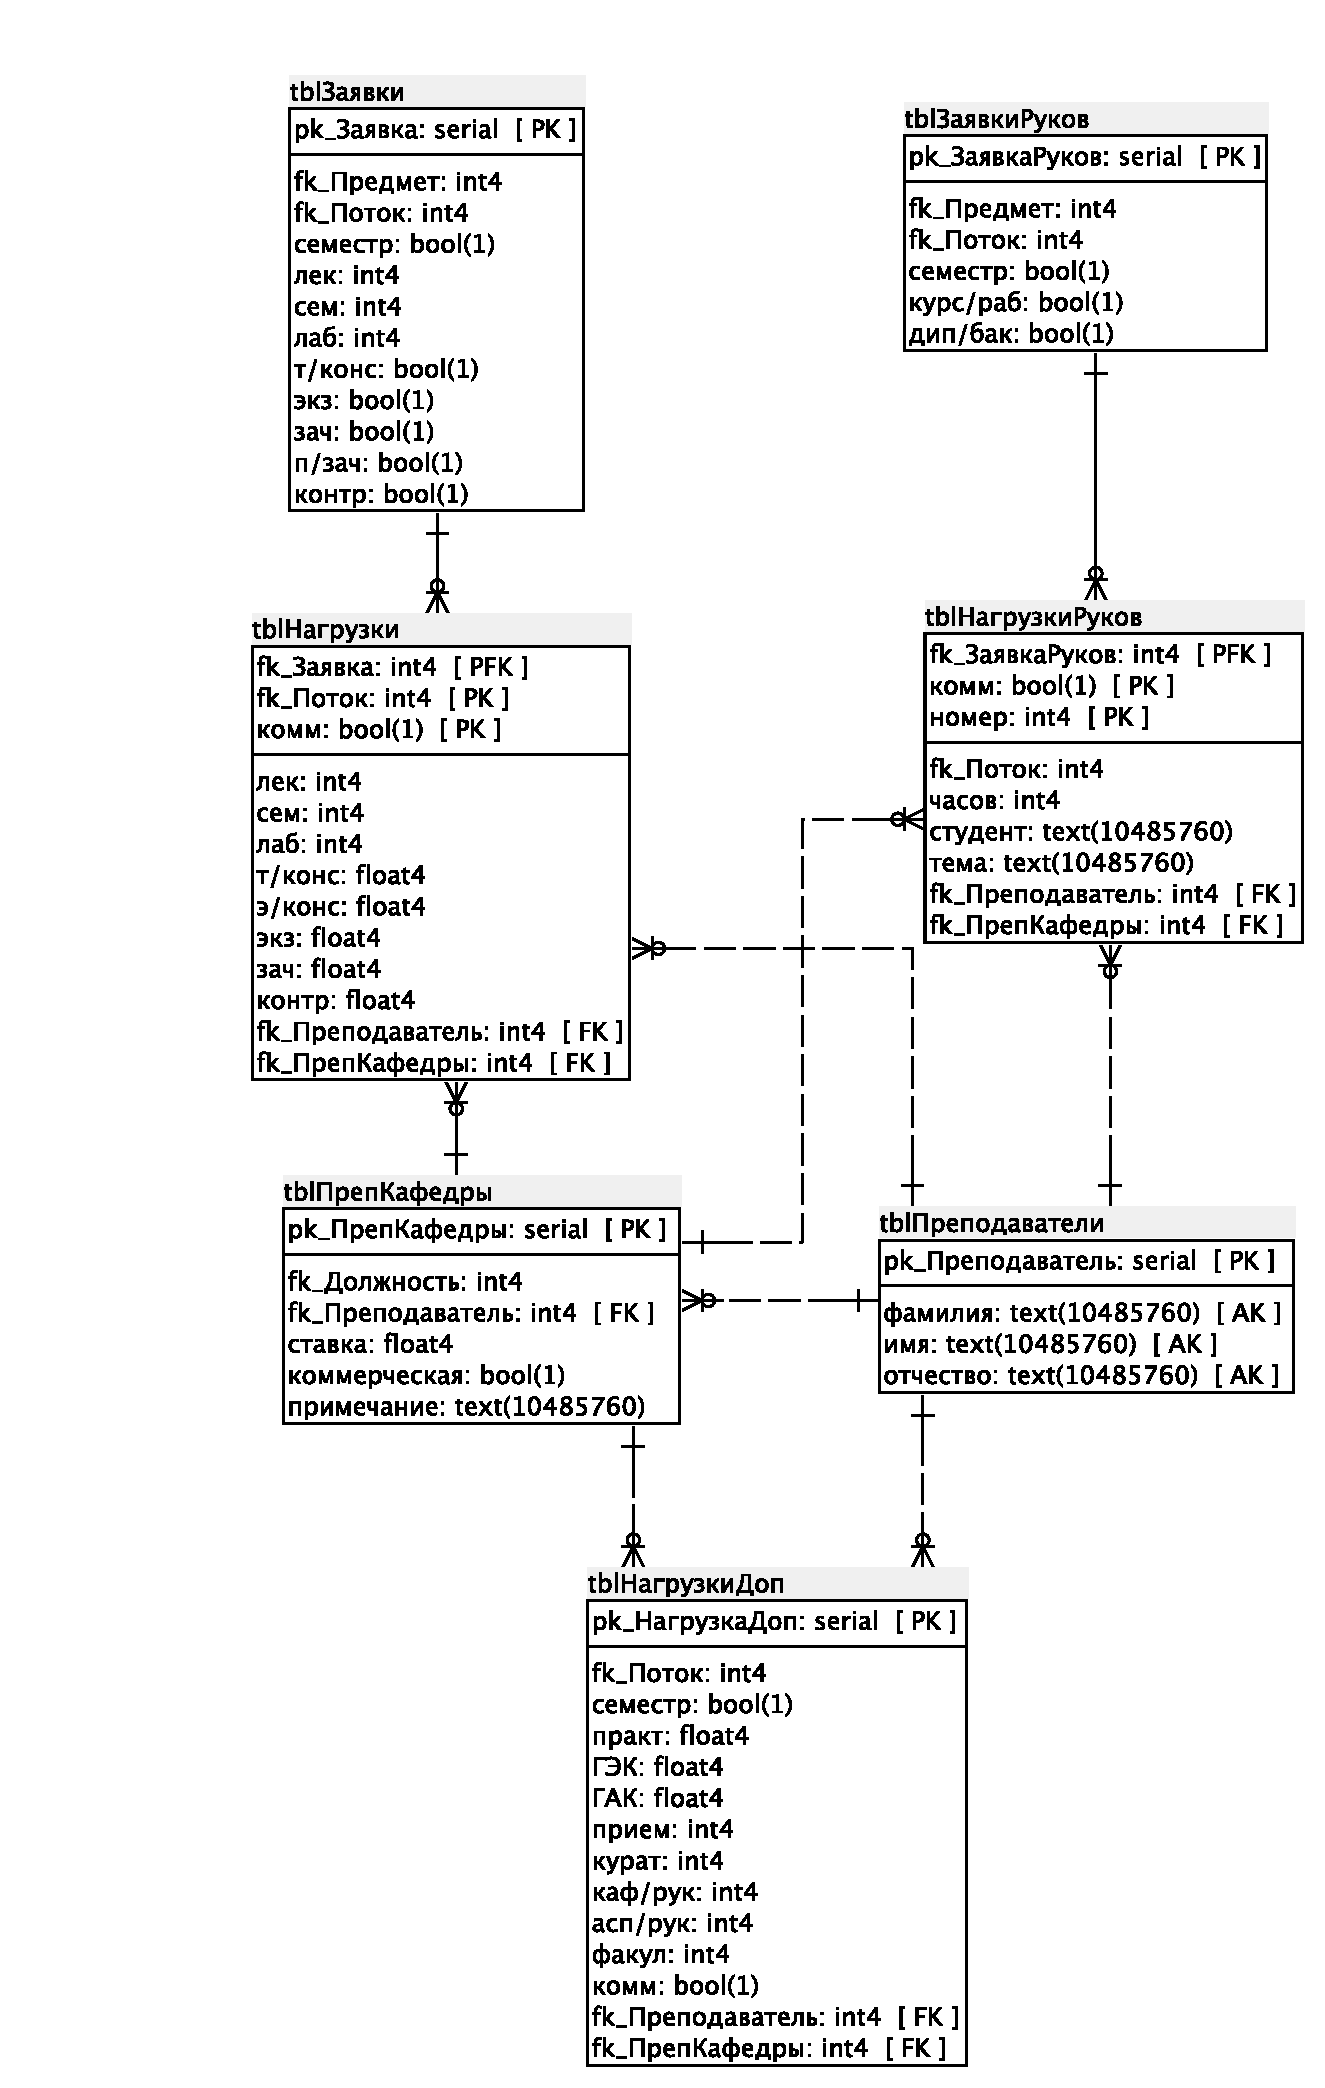
\includegraphics[scale=0.25]{db5}%
\end{center}
\end{frame}

\section{Библиотека PyQt4}
\begin{frame}
\begin{block}{Библиотека Qt4}
Qt4 -- популярная кроссплатформенная библиотека C++ для разработки GUI-приложений. Поддерживаемые операционные системы: Windows, Mac OS X, GNU/Linux и иные Unix-подобные системы. Особенности:
\begin{itemize}
 \item Виджеты, менеджеры размещений, стили
 \item Стандартные (и не очень) GUI-компоненты приложения
 \item Лёгкая коммуникация между компонентами (сигналы и слоты)
 \item Независимая система отображения (прозрачность, сглаживание, поддержка SVG)
 \item Поддержка баз данных и XML в русле идеологии MVC (модель-представление)
 \item Поддержка сетевых протоколов, многопоточности и др.
\end{itemize}
\end{block}
\begin{block}{PyQt}
PyQt4 -- привязка библиотеки Qt к языку Python, сочетающая в себе положительные стороны Qt и расширяющая её возможности высокоуровневыми особенностями Python.
\end{block}
\end{frame}

\section{Создания интрефейса пользователя к БД «кафедральная нагрузка»}

\begin{frame}
\frametitle{Редактирование tblСпециальности}
\begin{center}
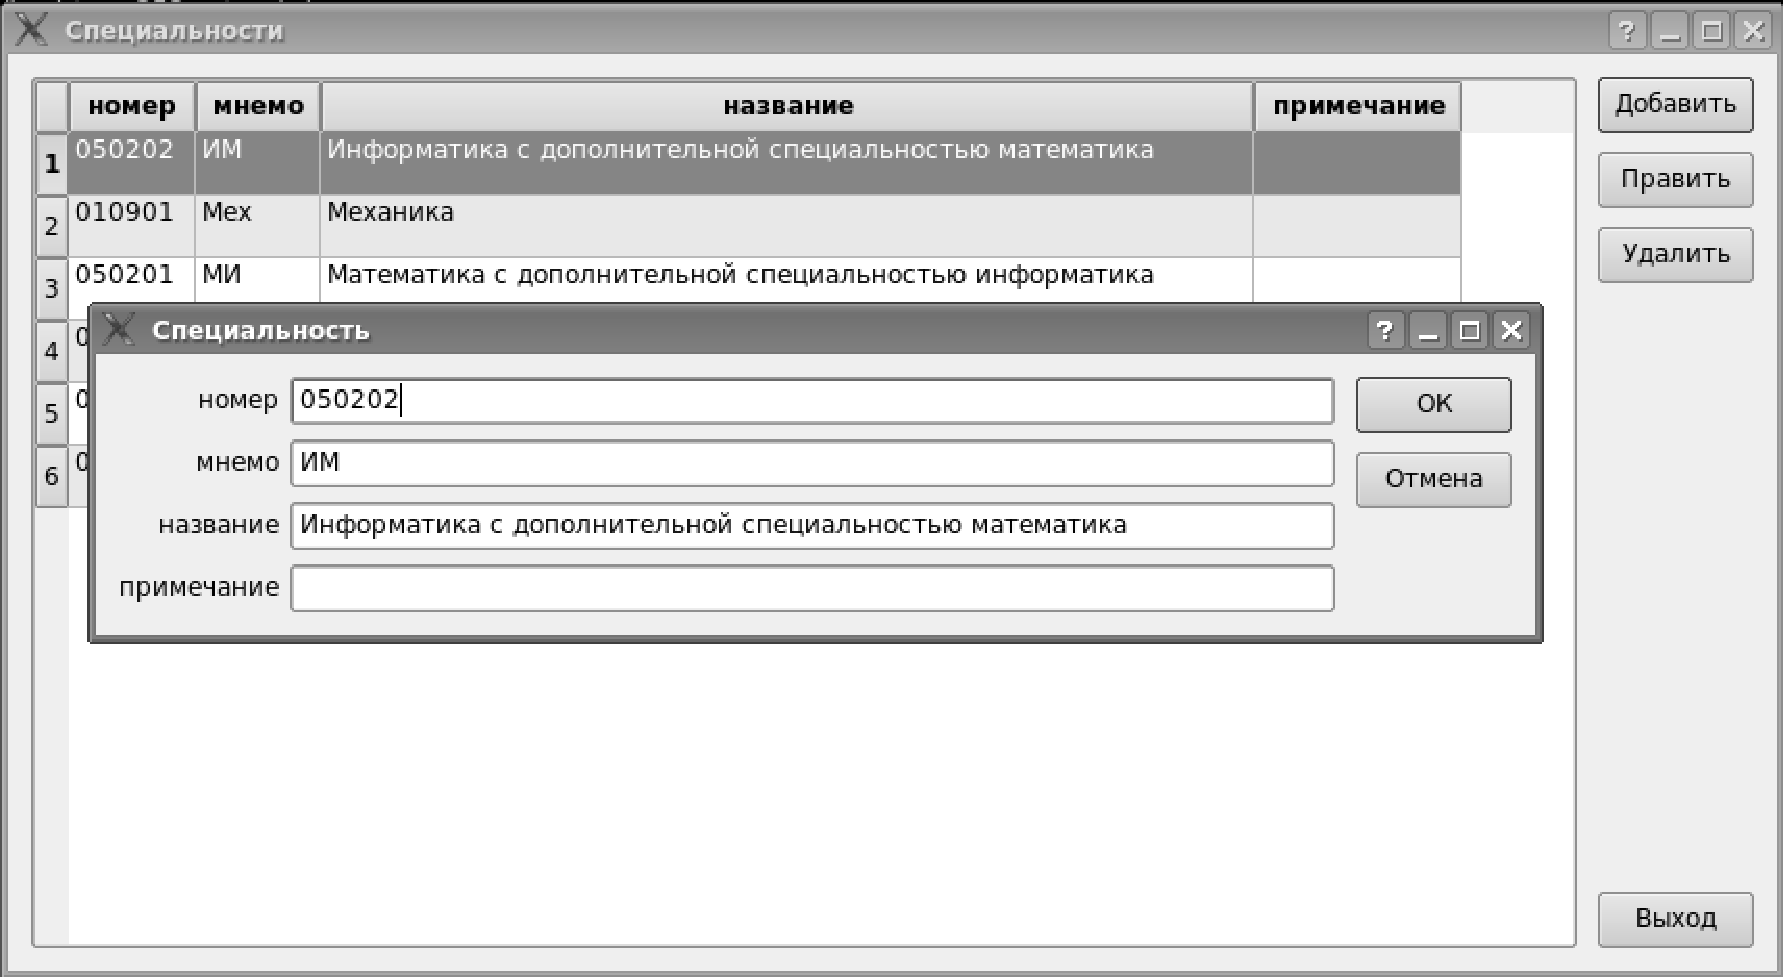
\includegraphics[width=1.0\textwidth]{tbl1}%
\end{center}
\end{frame}

\begin{frame}
\frametitle{Редактирование tblПодгруппы}
\begin{center}
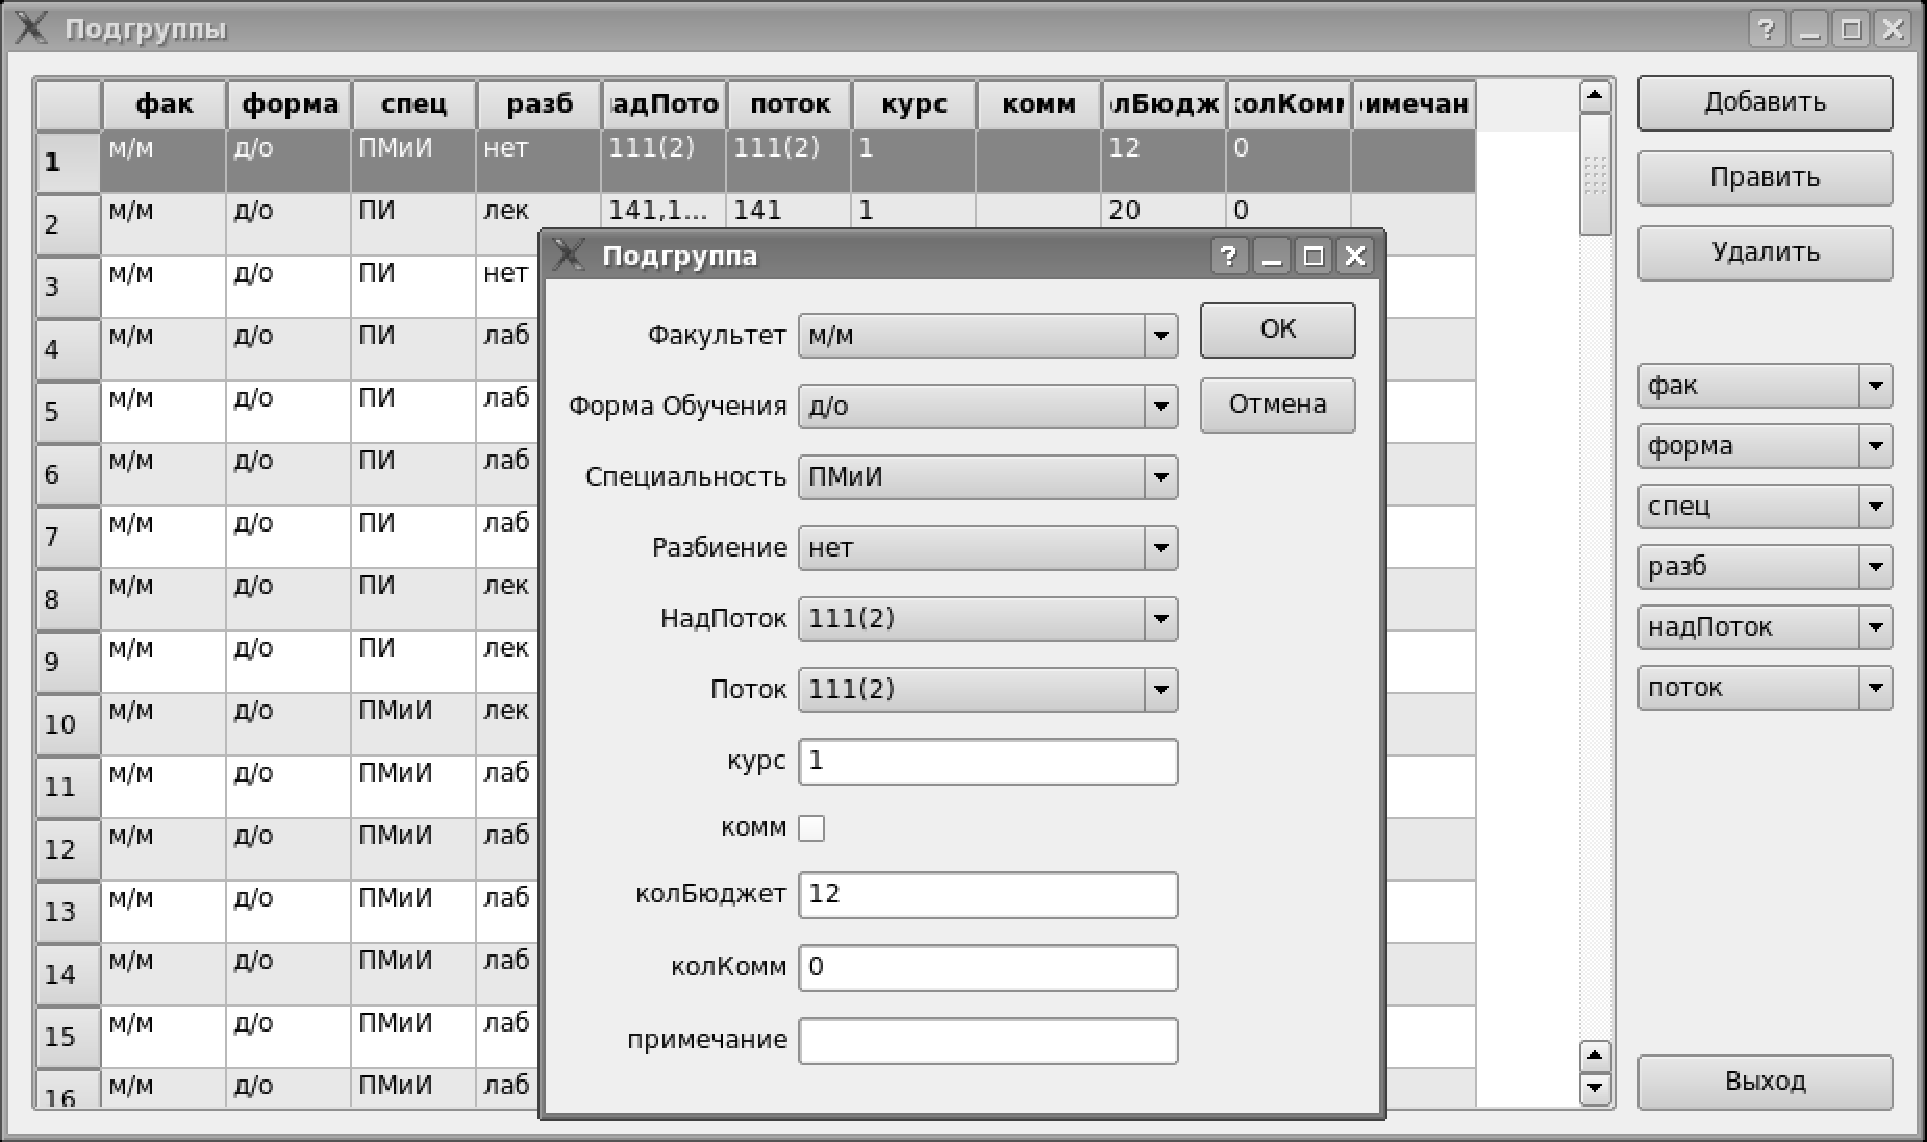
\includegraphics[width=1.0\textwidth]{tbl2}%
\end{center}
\end{frame}

\begin{frame}
\frametitle{Редактирование tblЗаявки}
\begin{center}
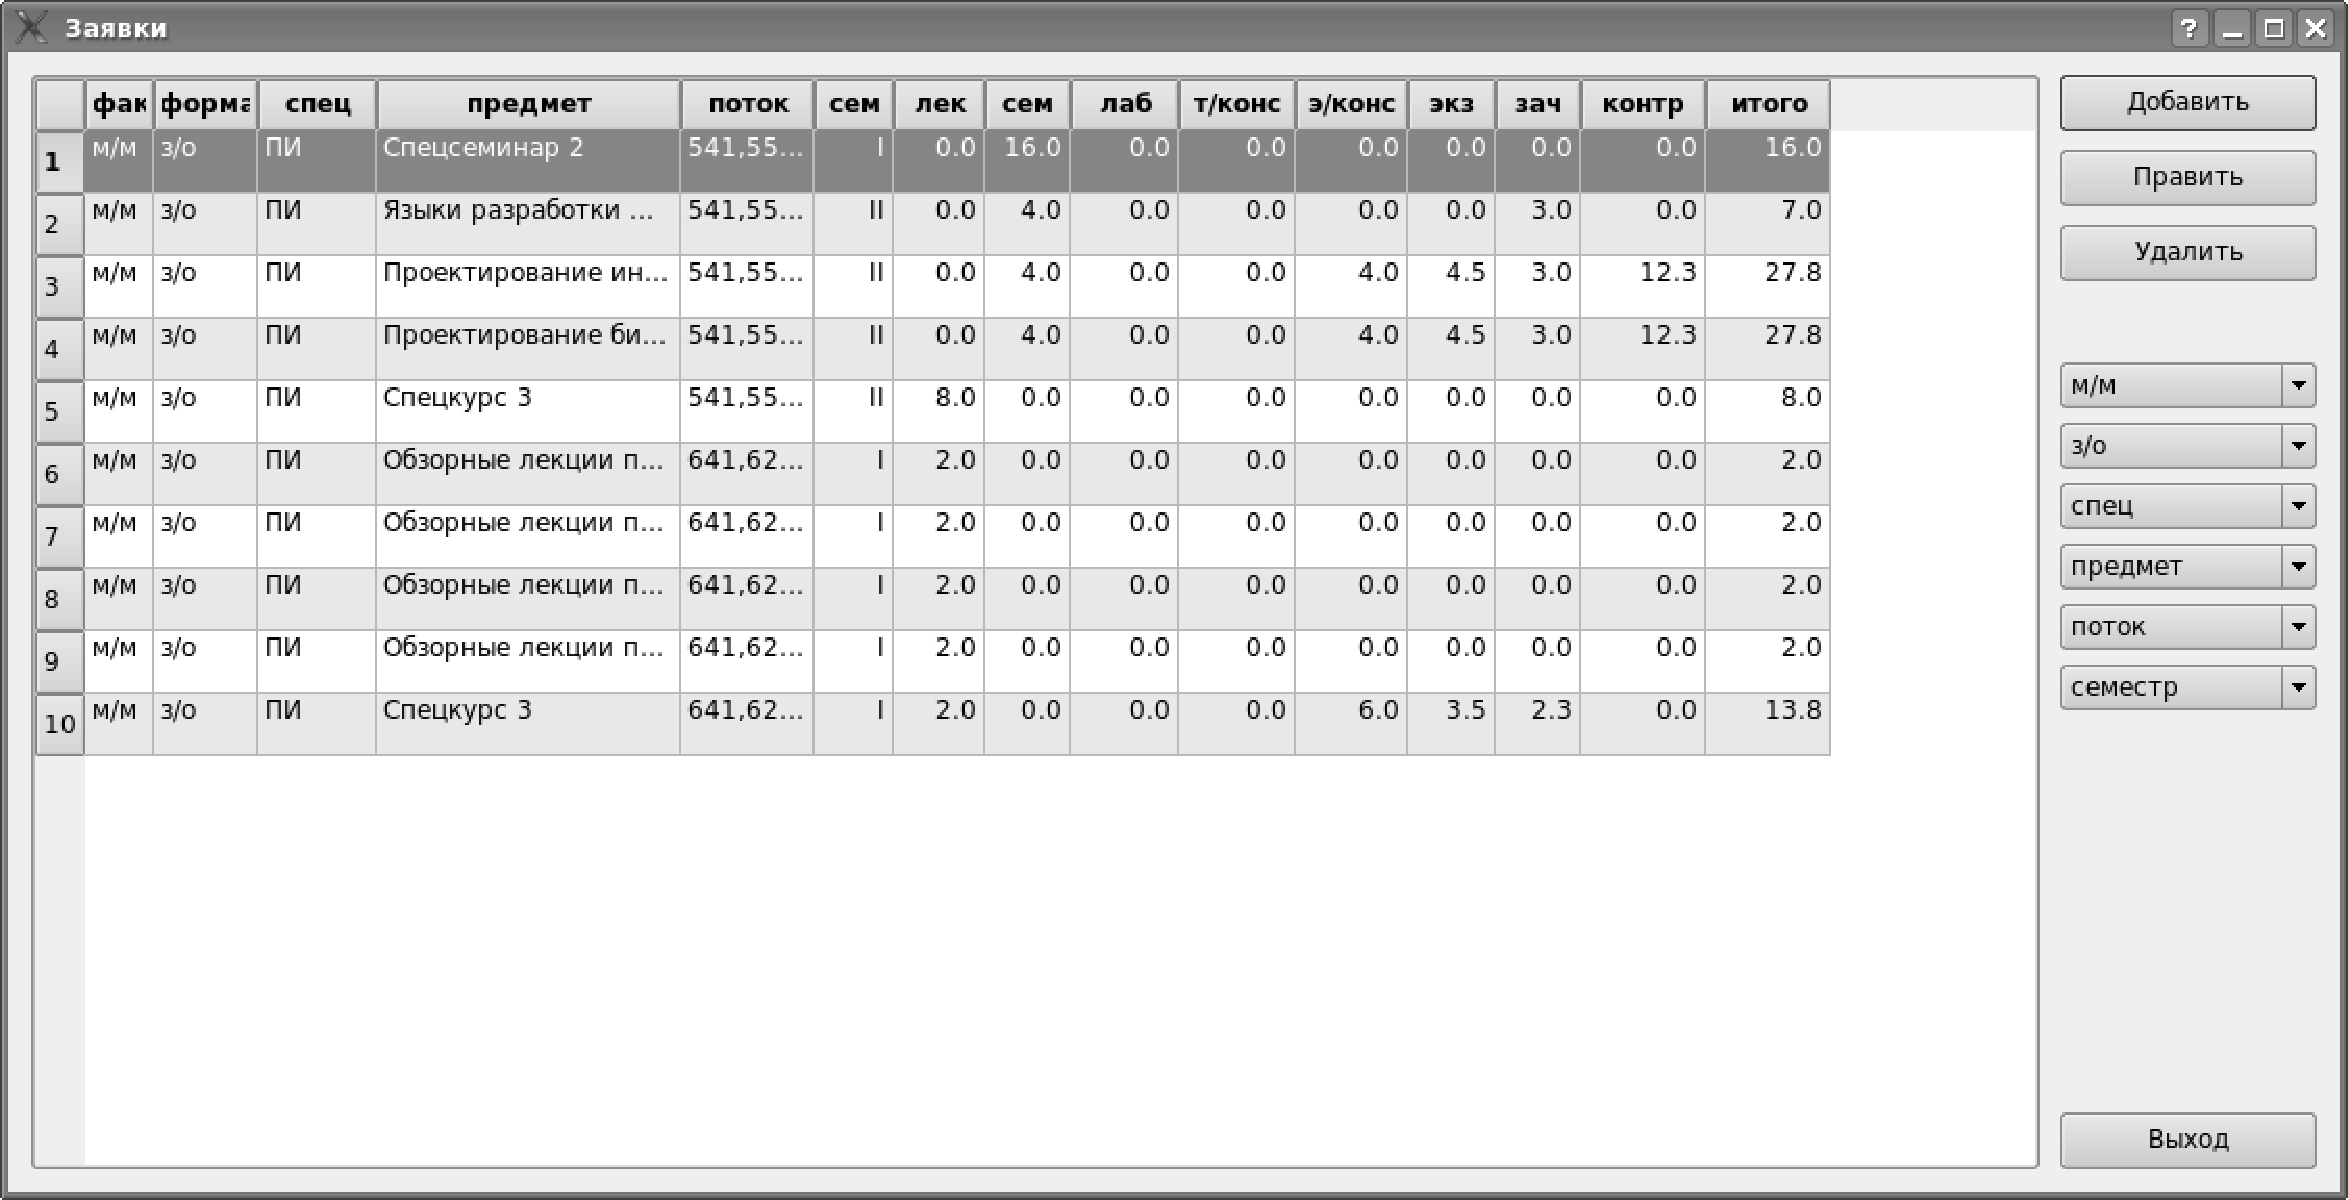
\includegraphics[width=1.0\textwidth]{tbl3}%
\end{center}
\end{frame}

\begin{frame}
\frametitle{Редактирование tblЗаявки}
\begin{center}
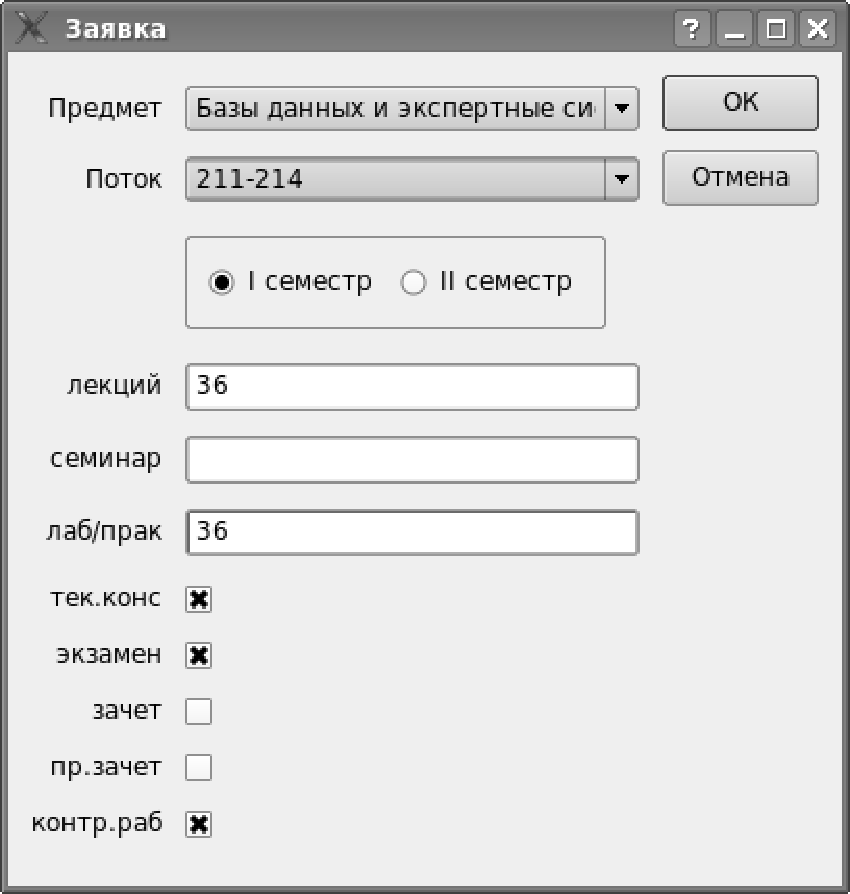
\includegraphics[scale=0.5]{tbl4}%
\end{center}
\end{frame}

\begin{frame}
\frametitle{Редактирование tblНагрузки}
\begin{center}
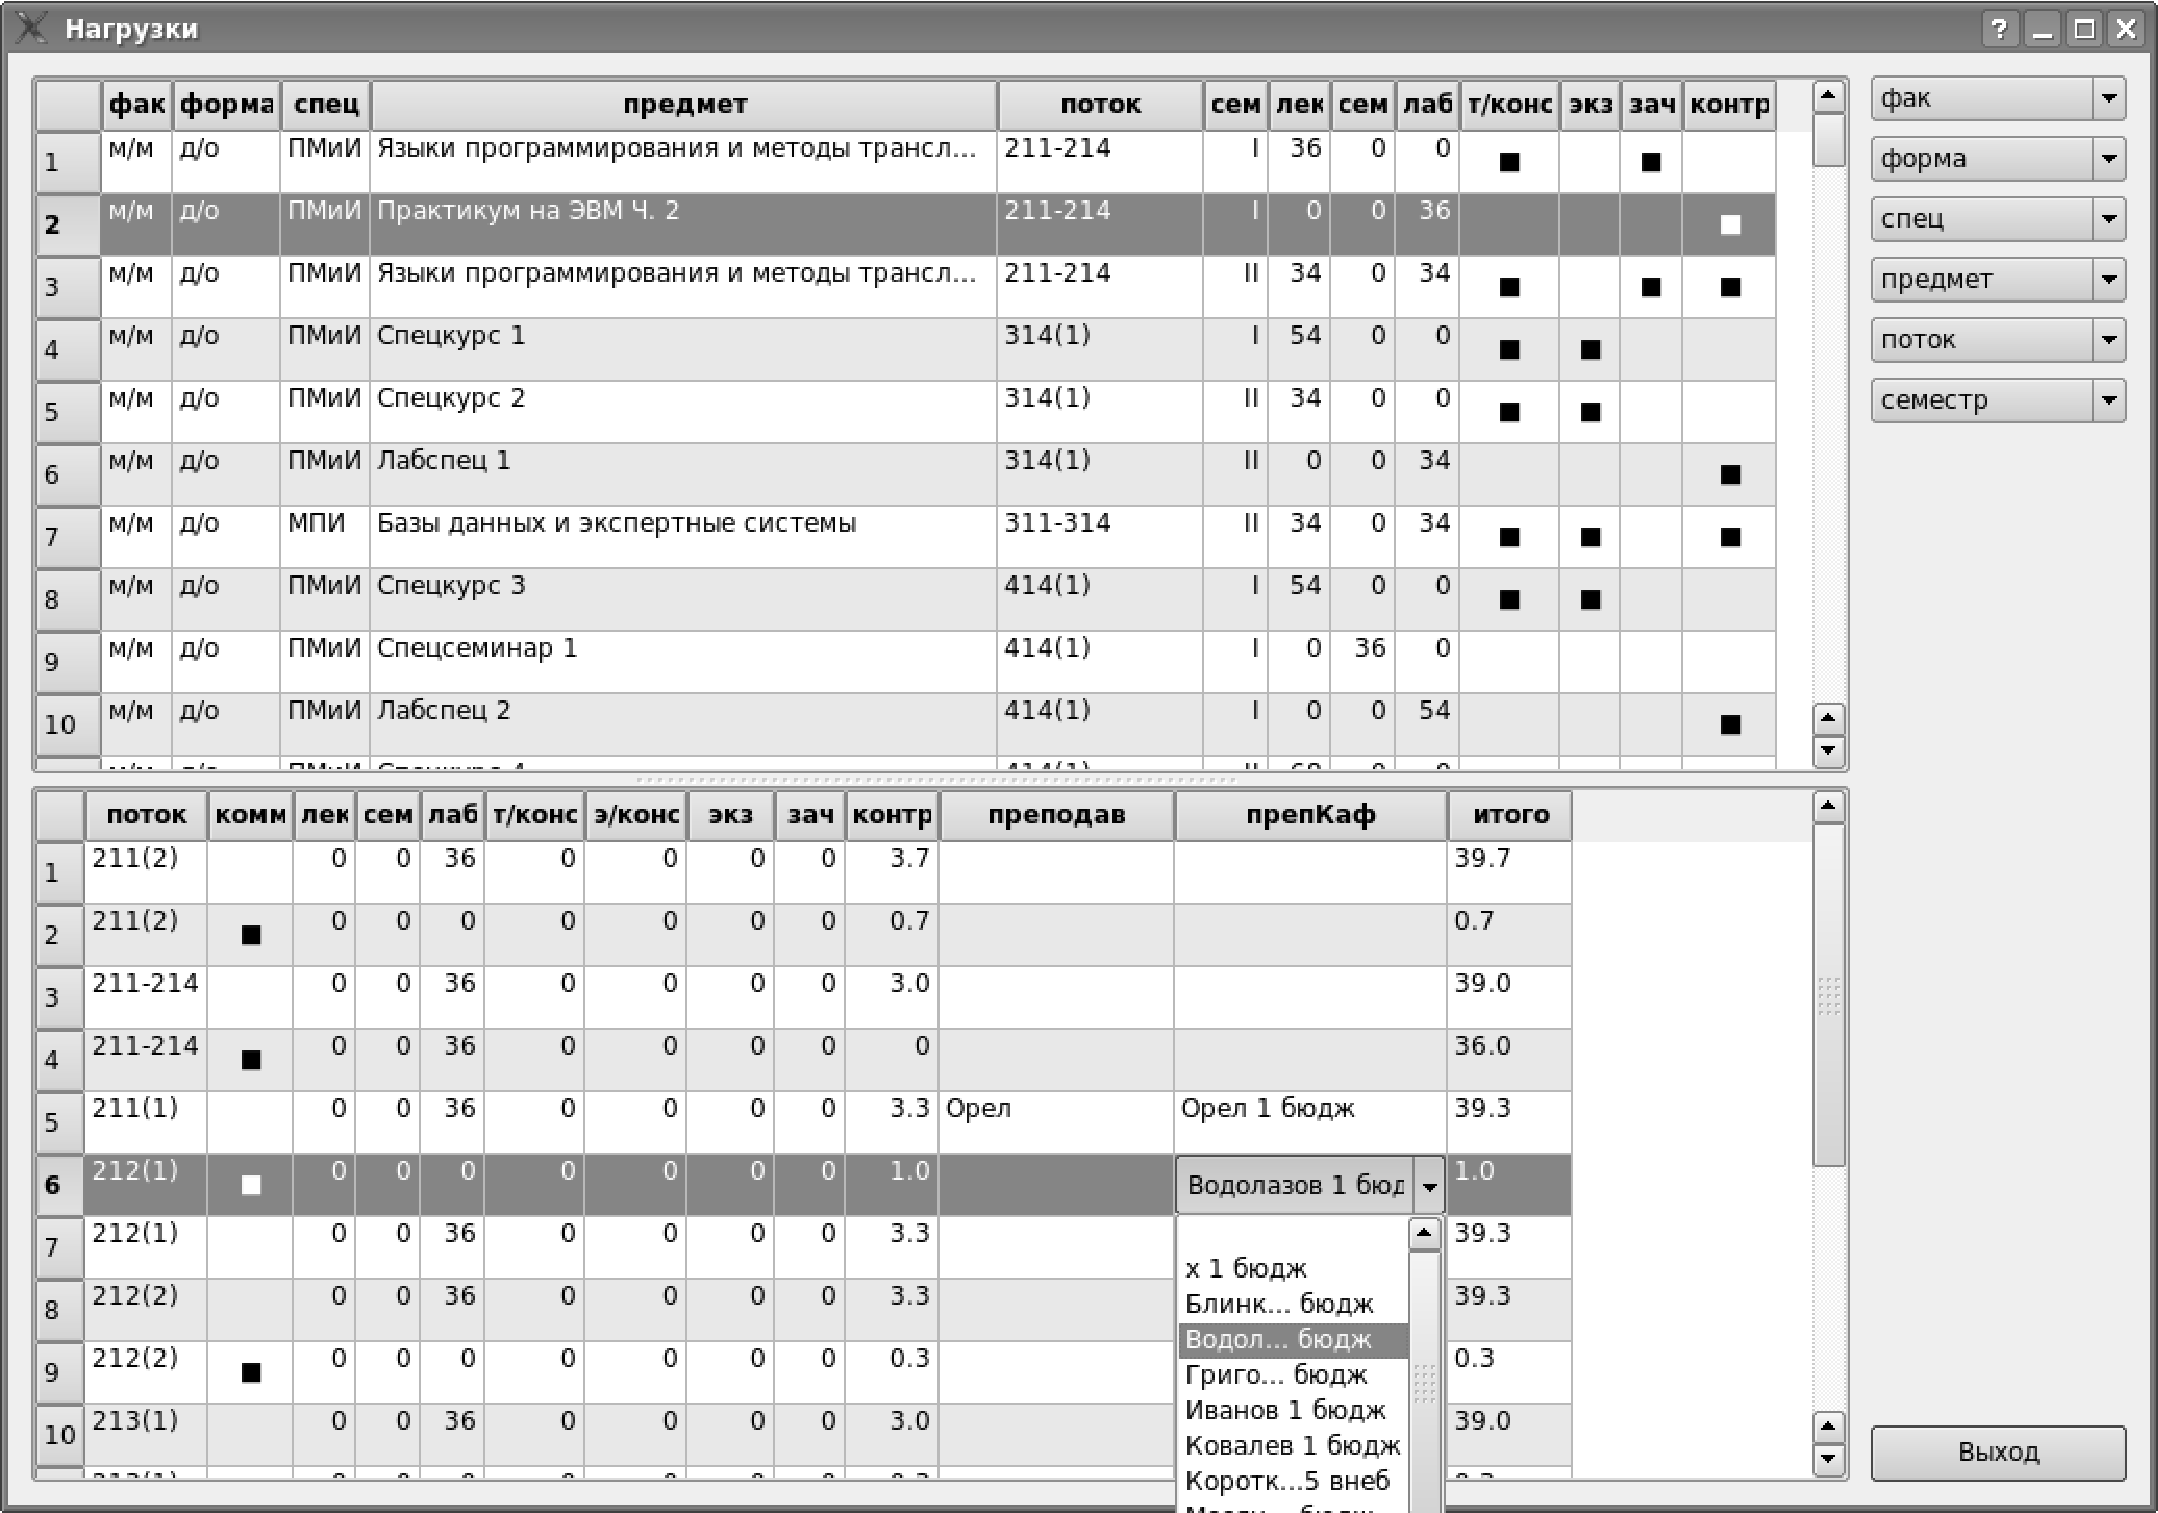
\includegraphics[width=0.9\textwidth]{tbl5}%
\end{center}
\end{frame}

\section{Заключение}
\begin{frame}
\frametitle{Заключение}
\begin{block}{В дипломной работе}
\begin{itemize}
 \item Рассмотрена работа библиотеки графического интерфейса пользователя \emph{PyQt4}.
 \item С ее помощью для БД «кафедральная нагрузка» сделан графический интерфейс пользователя.
 \item В настоящее время он успешно применяется на кафедре
 при составлении
кафедральной нагрузки. 
\end{itemize}
\end{block}
\end{frame}
\end{document}
